% ------------------------------------------------------------------------------
% TYPO3 CMS 6.2 LTS - What's New - Chapter « Backend Changes » (French version)
%
% @author	Paul Blondiaux <pblondiaux@sodifrance.fr>
% @author	Philippe Herault <philippe.herault@plan-net.fr>
% @license	Creative Commons BY-NC-SA 3.0
% @link		http://typo3.org/download/release-notes/whats-new/
% @language	French
% ------------------------------------------------------------------------------
% Chapter: Backend Changes
% ------------------------------------------------------------------------------

\section{Backend Changes}
\begin{frame}[fragile]
	\frametitle{Changements en Backend}

	\begin{center}\huge{Chapitre 3 :}\end{center}
	\begin{center}\huge{\color{typo3darkgrey}\textbf{Changements en Backend}}\end{center}

\end{frame}

% ------------------------------------------------------------------------------
% Autofocus
% ------------------------------------------------------------------------------
% http://forge.typo3.org/issues/49228

\begin{frame}[fragile]
	\frametitle{Changements en Backend}
	\framesubtitle{Connexion}

 	\begin{itemize}
		\item Positionnement automatique du curseur sur le champ utilisateur du formulaire de connexion\newline
			(Attribut HTML5 : \texttt{autofocus="autofocus"})
	\end{itemize}

	\begin{figure}
		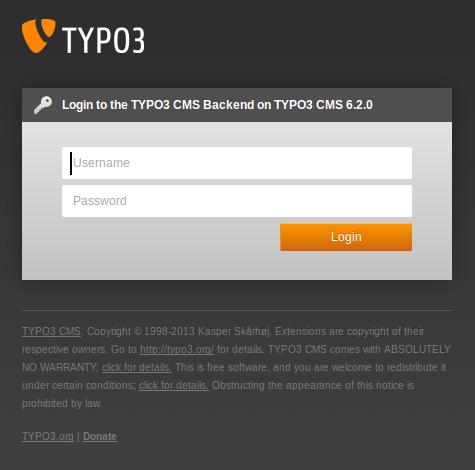
\includegraphics[width=0.4\linewidth]{Images/BackendChanges/BackendLogin.png}
	\end{figure}

\end{frame}

% ------------------------------------------------------------------------------
% Visual Appearance
% ------------------------------------------------------------------------------
% http://forge.typo3.org/issues/48376

\begin{frame}[fragile]
	\frametitle{Changements en Backend}
	\framesubtitle{Aspect visuel (1)}

	\begin{columns}[T]

		\begin{column}{.5\textwidth}
			\begin{itemize}
				\item Amélioration de l'utilisabilité par l'animation du backend
				\item Marges entre les modules (colonne gauche) augmentées
				\item En se basant sur une grille de 12px, laquelle a été doublée
			\end{itemize}

			\advance\leftskip+3.8cm

			\smaller
				A gauche : TYPO3 4.5\newline
				A droite : TYPO3 6.2
			\normalsize
		\end{column}

		\begin{column}{.5\textwidth}
			\begin{figure}\vspace*{-0.4cm}
				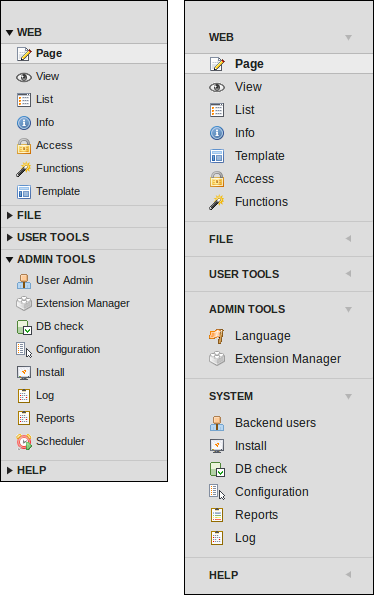
\includegraphics[width=0.6\linewidth]{Images/BackendChanges/VisualAppearance.png}
			\end{figure}
		\end{column}

	\end{columns}

\end{frame}

% ------------------------------------------------------------------------------
% Visual Appearance
% ------------------------------------------------------------------------------

\begin{frame}[fragile]
	\frametitle{Changements en Backend}
	\framesubtitle{Aspect visuel (2)}

	\begin{columns}[T]

		\begin{column}{.5\textwidth}

			\begin{itemize}
				\item Les modules de la colonne de gauche ont été restructurés
				\item Le module « ADMINTOOLS » est divisé en deux parties :

					\begin{itemize}
						\item \textbf{ADMINTOOLS} (« Langues » et « Gestionnaire d'extensions »)
						\item \textbf{SYSTEM} (outils de bas niveau, qui ne nécessitent pas l'affichage de l'arborescence)
					\end{itemize}

				\item Le module « TypoScript Help » a été supprimé (obsolète)

			\end{itemize}

		\end{column}

		\begin{column}{.5\textwidth}
			\begin{figure}\vspace*{-0.4cm}
				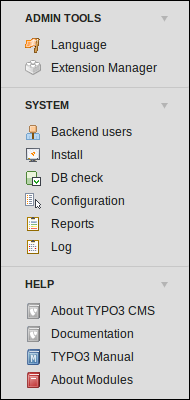
\includegraphics[width=0.35\linewidth]{Images/BackendChanges/AdminTools.png}
			\end{figure}
		\end{column}

	\end{columns}

\end{frame}

% ------------------------------------------------------------------------------
% Visual Appearance
% ------------------------------------------------------------------------------
% http://forge.typo3.org/issues/36017

\begin{frame}[fragile]
	\frametitle{Changements en Backend}
	\framesubtitle{Aspect visuel (3)}

	\begin{itemize}
		\item Les titres \texttt{<h1>} dans la zone principale utilisent la police « Share »
	\end{itemize}

	\begin{figure}
		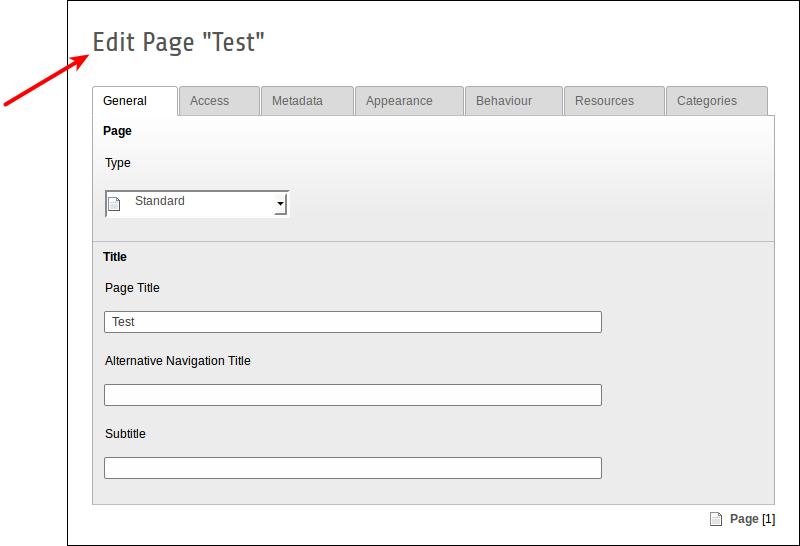
\includegraphics[width=0.6\linewidth]{Images/BackendChanges/ConsistantFont.png}
	\end{figure}

\end{frame}

% ------------------------------------------------------------------------------
% Visual Appearance
% ------------------------------------------------------------------------------
% http://forge.typo3.org/issues/41631

\begin{frame}[fragile]
	\frametitle{Changements en Backend}
	\framesubtitle{Aspect visuel (4)}

	\begin{itemize}
		\item Le module « Rapports » présente une nouvelle icône
	\end{itemize}

	\begin{figure}
		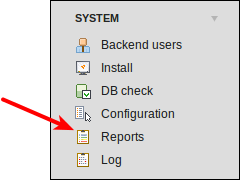
\includegraphics[width=0.35\linewidth]{Images/BackendChanges/ModuleReportsIcon.png}
	\end{figure}

\end{frame}

% ------------------------------------------------------------------------------
% Drag&Drop File Upload in Filelist (FAL)
% ------------------------------------------------------------------------------
% http://forge.typo3.org/issues/47005

\begin{frame}[fragile]
	\frametitle{Changements en Backend}
	\framesubtitle{Chargement de fichier en « Drag\&Drop » (1)}

	\begin{itemize}
		\item Un chargement de fichier en « Drag\&Drop » HTML5 a été implémenté dans le module « Fichiers »
	\end{itemize}

	\begin{figure}
		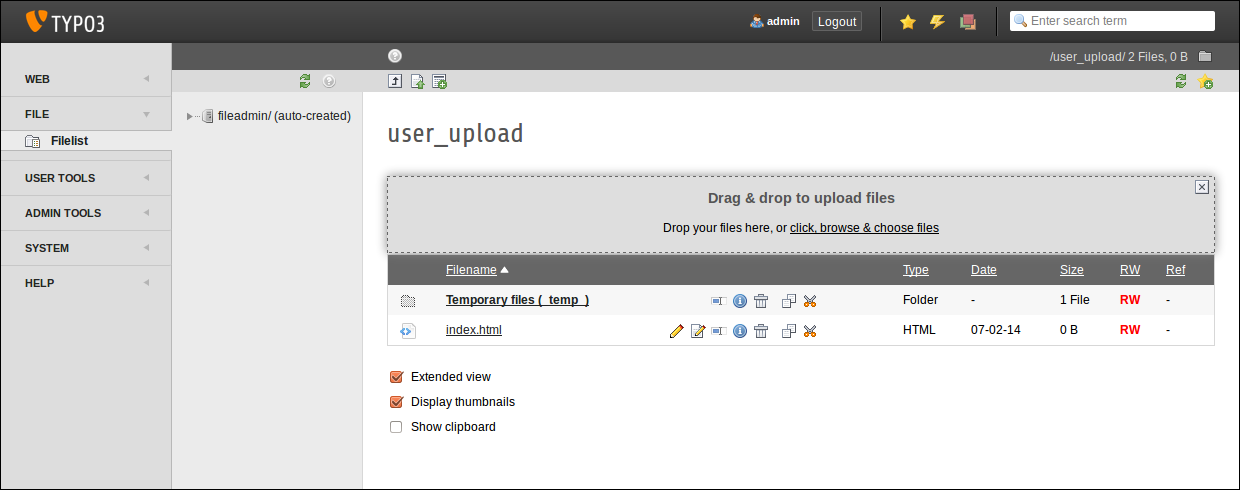
\includegraphics[width=0.95\linewidth]{Images/BackendChanges/DragDropFileUpload.png}
	\end{figure}

\end{frame}

% ------------------------------------------------------------------------------
% Drag&Drop File Upload Via Content Elements
% (slide added in March 2014)
% ------------------------------------------------------------------------------

\begin{frame}[fragile]
	\frametitle{Changements en Backend}
	\framesubtitle{Chargement de fichier en « Drag\&Drop » (2)}

	\begin{itemize}
		\item ...et dans les éléments de contenu (bouton: « Select \& upload files »)

	\end{itemize}

	\begin{figure}
		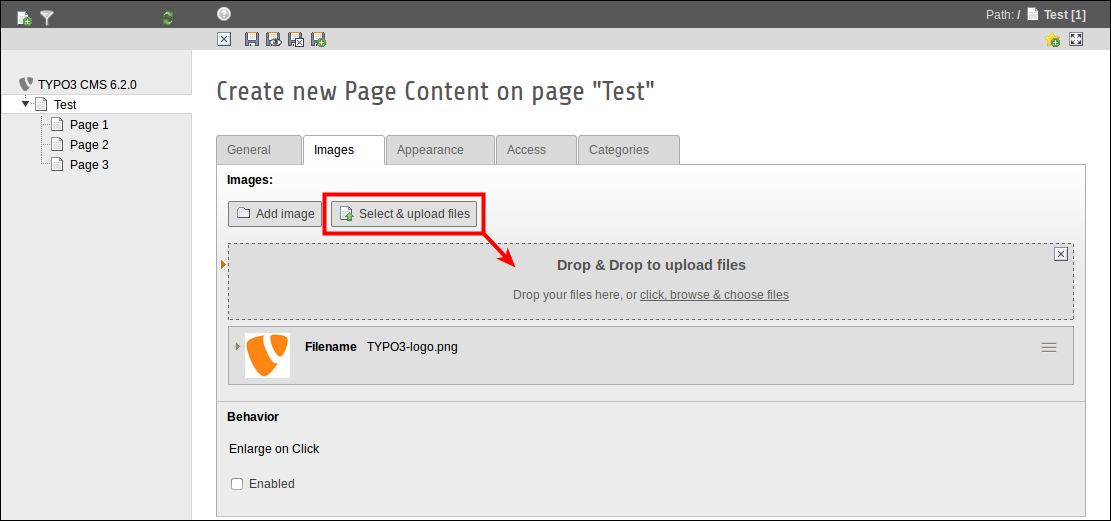
\includegraphics[width=0.95\linewidth]{Images/BackendChanges/SelectAndUploadFiles.png}
	\end{figure}

\end{frame}

% ------------------------------------------------------------------------------
% Backend Users
% ------------------------------------------------------------------------------
% http://forge.typo3.org/issues/43053

\begin{frame}[fragile]
	\frametitle{Changements en Backend}
	\framesubtitle{Utilisabilité : liste des utilisateurs Backend}

	\begin{itemize}
		\item Le nom d'utilisateur et le nom « réel » sont affichés (première colonne en vue liste)
		\item Cliquer sur le nom de l'utilisateur pour éditer son enregistrement
		\item Un bouton « effacer » a été ajouté dans la vue liste
	\end{itemize}

	\begin{figure}
		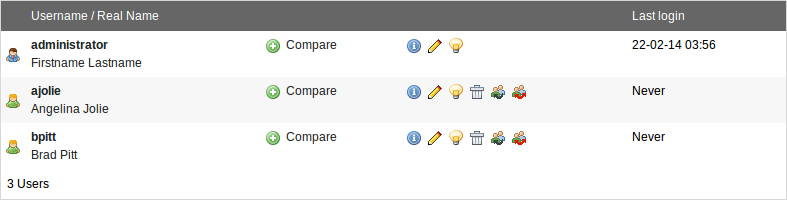
\includegraphics[width=0.95\linewidth]{Images/BackendChanges/BackendUserList.png}
	\end{figure}

\end{frame}

% ------------------------------------------------------------------------------
% Live Search
% ------------------------------------------------------------------------------
% http://forge.typo3.org/issues/35358

\begin{frame}[fragile]
	\frametitle{Changements en Backend}
	\framesubtitle{Recherche en temps réel (1)}

	\begin{itemize}
		\item Une bulle affiche l'UID et le PID dans la recherche « livesearch »
		\item Lorsqu'après une recherche, le formulaire d'édition est à nouveau fermé, la vue liste est affichée (et non une page vide)
	\end{itemize}

	\begin{figure}
		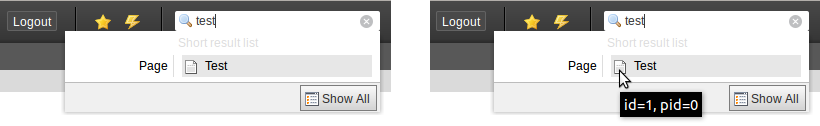
\includegraphics[width=0.8\linewidth]{Images/BackendChanges/LiveSearchTooltip.png}
	\end{figure}

\end{frame}

% ------------------------------------------------------------------------------
% Live Search
% ------------------------------------------------------------------------------

\begin{frame}[fragile]
	\frametitle{Changements en Backend}
	\framesubtitle{Recherche en temps réel (2)}

	\begin{itemize}
		\item Dans TYPO3 < 6.2, pour les pages, seuls les champs \texttt{titre} et \texttt{uid} sont recherchés
		\item Dans TYPO3 >= 6.2, le champ \texttt{alias} peut être ajouté à la recherche\newline
			(UserTSconfig : \texttt{options.pageTree.searchInAlias = 1})
	\end{itemize}

	\begin{figure}
		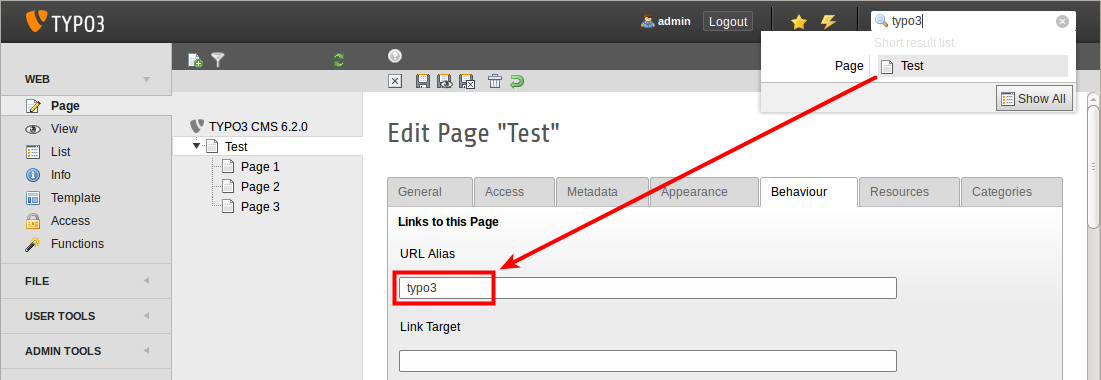
\includegraphics[width=0.95\linewidth]{Images/BackendChanges/LiveSearchInAlias.png}
	\end{figure}

\end{frame}

% ------------------------------------------------------------------------------
% File Abstraction Layer
% ------------------------------------------------------------------------------

\begin{frame}[fragile]
	\frametitle{Changements en Backend}
	\framesubtitle{File Abstraction Layer}

	\begin{itemize}
		\item Le nom et le titre du fichier sont affichés dans l'en-tête de l'enregistrement FAL
	\end{itemize}

	\begin{figure}
		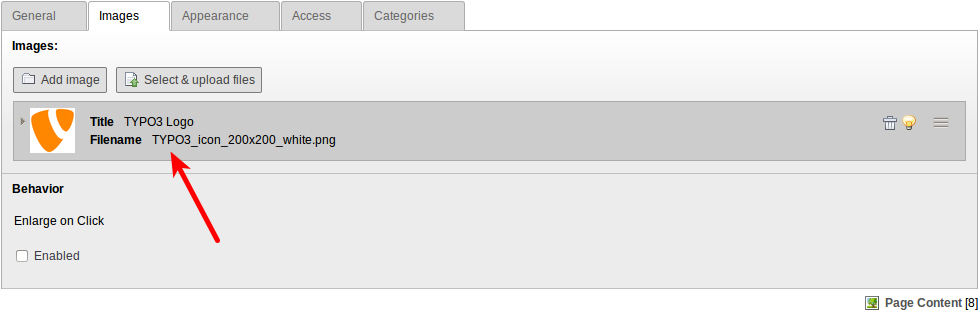
\includegraphics[width=0.95\linewidth]{Images/BackendChanges/FalTitleAndFilename.png}
	\end{figure}

\end{frame}

% ------------------------------------------------------------------------------
% File Abstraction Layer
% ------------------------------------------------------------------------------

\begin{frame}[fragile]
	\frametitle{Changements en Backend}
	\framesubtitle{File Abstraction Layer (EXT:filemetadata)}

	\begin{itemize}
		\item L'extension système : « filemetadata » ajoute des onglets affichant les méta-données
			(l'extension est livrée avec le cœur mais non installée par défaut)
	\end{itemize}

	\begin{figure}
		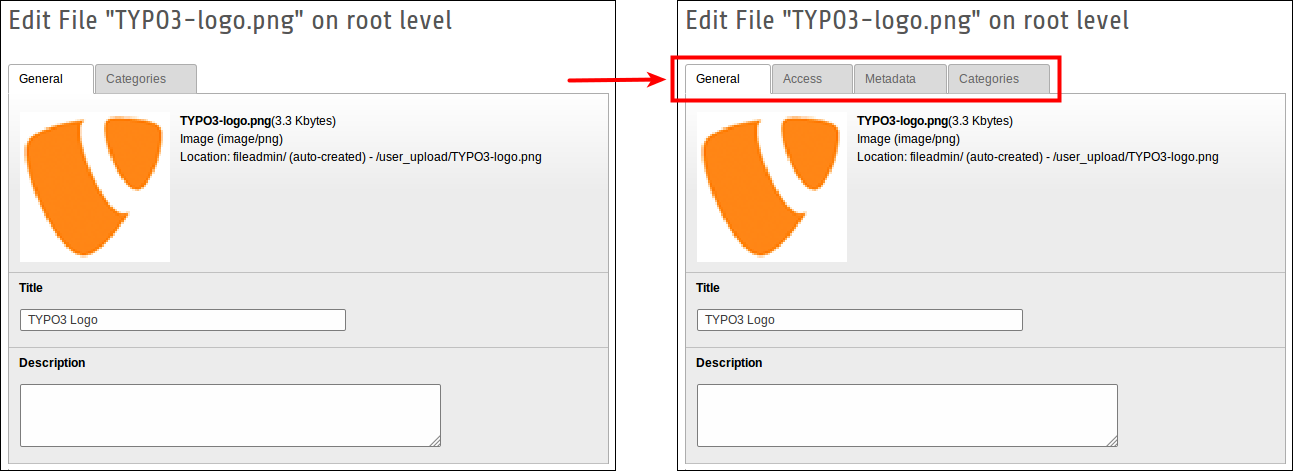
\includegraphics[width=0.95\linewidth]{Images/BackendChanges/FileMetaDataTabs.png}
	\end{figure}

\end{frame}

% ------------------------------------------------------------------------------
% File Abstraction Layer
% ------------------------------------------------------------------------------

\begin{frame}[fragile]

	\frametitle{Changements en Backend}
	\framesubtitle{File Abstraction Layer (EXT:filemetadata)}

	\begin{figure}
		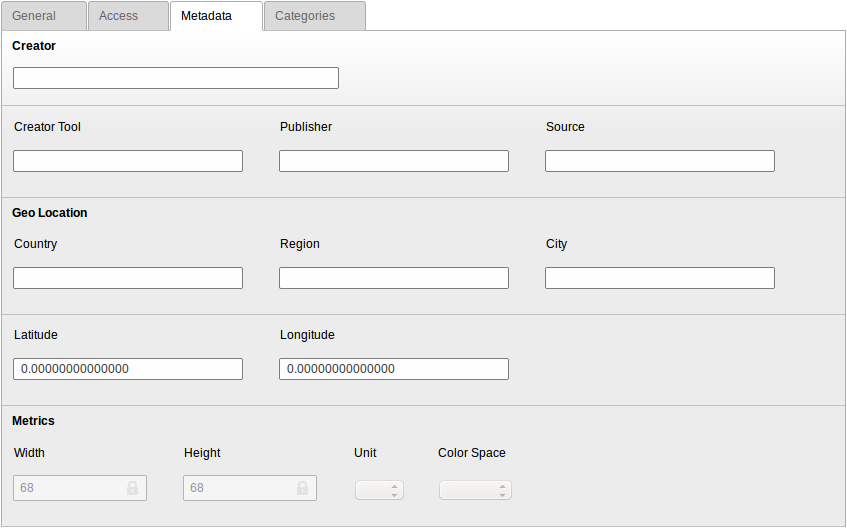
\includegraphics[width=0.8\linewidth]{Images/BackendChanges/FileMetaData.png}
	\end{figure}

\end{frame}

% ------------------------------------------------------------------------------
% File Abstraction Layer
% ------------------------------------------------------------------------------

\begin{frame}[fragile]
	\frametitle{Changements en Backend}
	\framesubtitle{File Abstraction Layer}

	\begin{itemize}
		\item Il est maintenant possible de traduire les métadonnées du FAL dans\newline
				les langues Frontend
	\end{itemize}

	\begin{figure}
		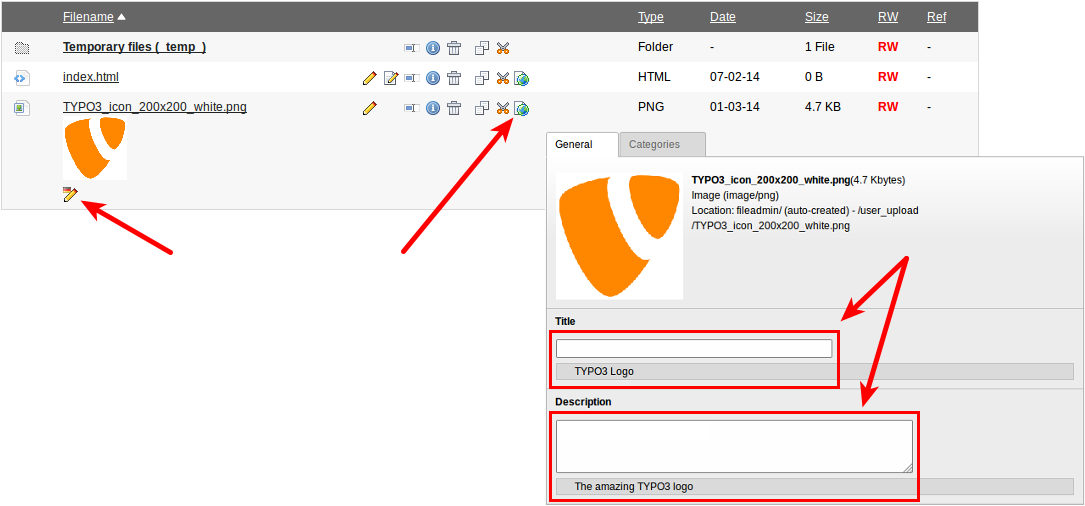
\includegraphics[width=0.95\linewidth]{Images/BackendChanges/FalTranslateMetaData.png}
	\end{figure}

\end{frame}

% ------------------------------------------------------------------------------
% Module : Documentation
% ------------------------------------------------------------------------------

\begin{frame}[fragile]
	\frametitle{Changements en Backend}
	\framesubtitle{Module : Documentation}

	\begin{columns}[T]

		\begin{column}{.5\textwidth}
			\begin{itemize}
				\item « Documentation » permet à l'utilisateur BE de télécharger et de visualiser les manuels
				\item Toute nouvelle installation TYPO3 charge ce module par défaut
				\item « Télécharger une documentation » permet de télécharger les manuels (voir l'illustration)
				\item Utilisez le gestionnaire d'extensions pour charger le module « Documentation » dans une instance mise à jour
			\end{itemize}
		\end{column}

		\begin{column}{.5\textwidth}
			\begin{figure}\vspace*{-0.4cm}
				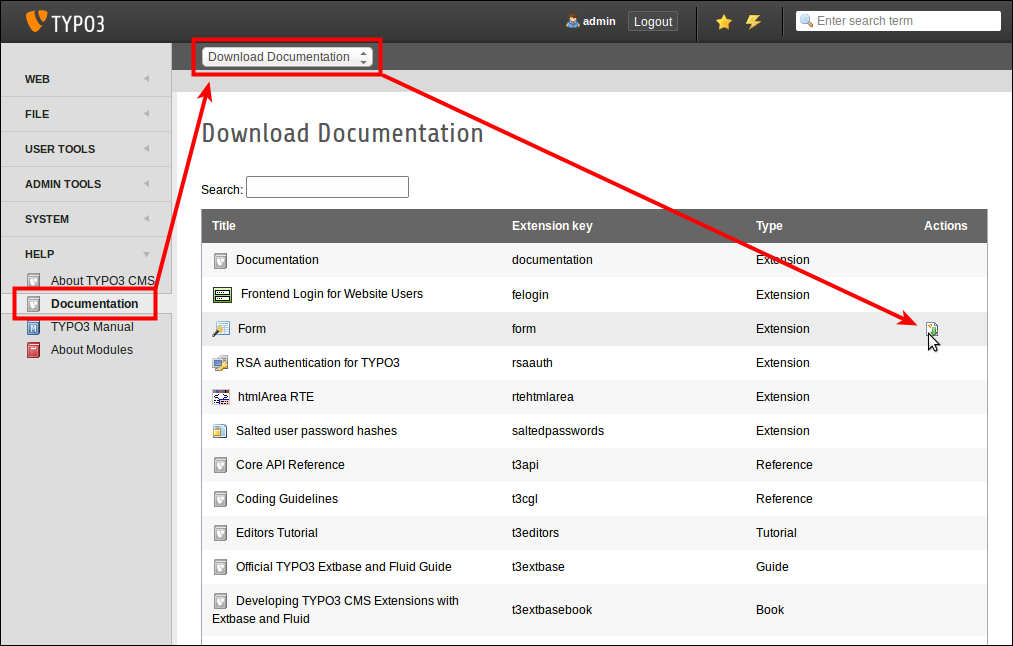
\includegraphics[width=1\linewidth]{Images/BackendChanges/DownloadDocumentation.png}
			\end{figure}
		\end{column}

	\end{columns}

\end{frame}

% ------------------------------------------------------------------------------
% Module : Documentation
% ------------------------------------------------------------------------------

\begin{frame}[fragile]
	\frametitle{Changements en Backend}
	\framesubtitle{Module : Documentation}

	\begin{itemize}
		\item La fonction « Show Documentation » affiche les manuels téléchargés
	\end{itemize}

	\begin{figure}
		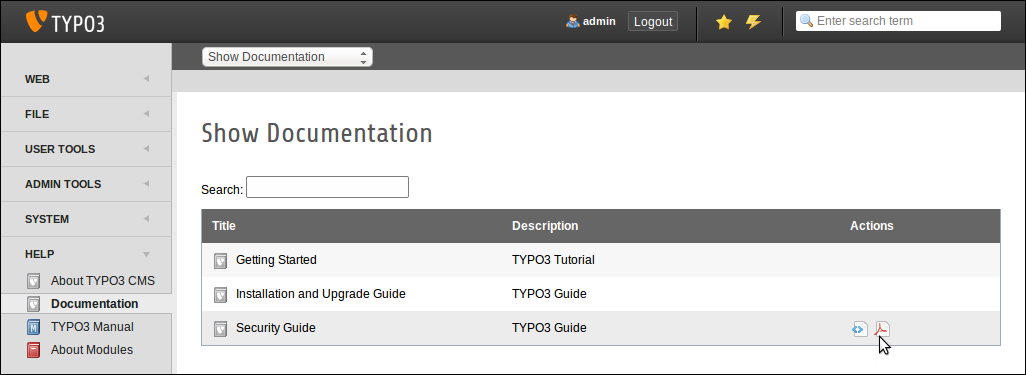
\includegraphics[width=0.95\linewidth]{Images/BackendChanges/ShowDocumentation.png}
	\end{figure}

\end{frame}

% ------------------------------------------------------------------------------
% Removed : TypoScript Help
% ------------------------------------------------------------------------------
% http://forge.typo3.org/issues/47931

\begin{frame}[fragile]
	\frametitle{Changements en Backend}
	\framesubtitle{Module supprimé : TypoScript Help}

 	\begin{itemize}
		\item L'extension : tsconfig\_help (« TSconfig Quick Reference ») a été enlevée\newline
		\small(Informations périmées et plus maintenues depuis la version 4.1 de TYPO3)
	\end{itemize}

	\begin{figure}
		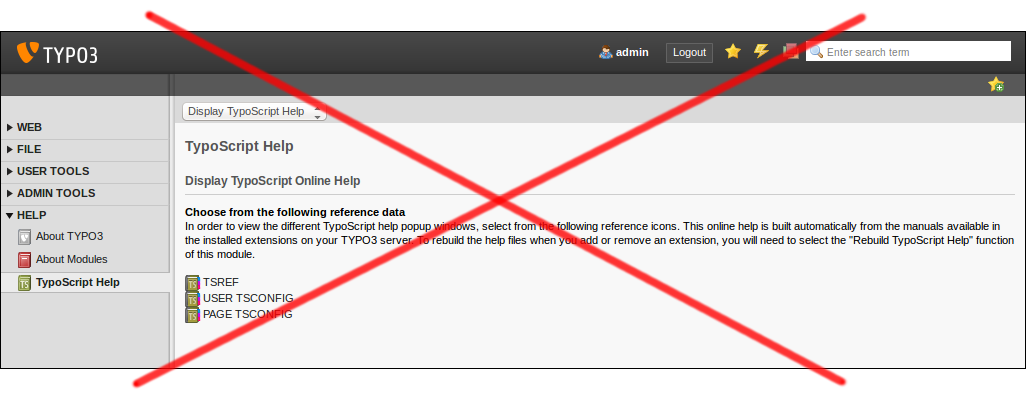
\includegraphics[width=0.95\linewidth]{Images/BackendChanges/TypoScriptHelpRemovedCrossed.png}
	\end{figure}

\end{frame}


% ------------------------------------------------------------------------------
% Scheduler
% ------------------------------------------------------------------------------

\begin{frame}[fragile]
	\frametitle{Changements en Backend}
	\framesubtitle{Planificateur (1)}

	\begin{itemize}
		\item Suppression d'une tâche possible en vue édition\newline
			(dans TYPO3 < 6.2, la fonction n'apparaissait qu'en mode liste)
	\end{itemize}

	\begin{figure}
		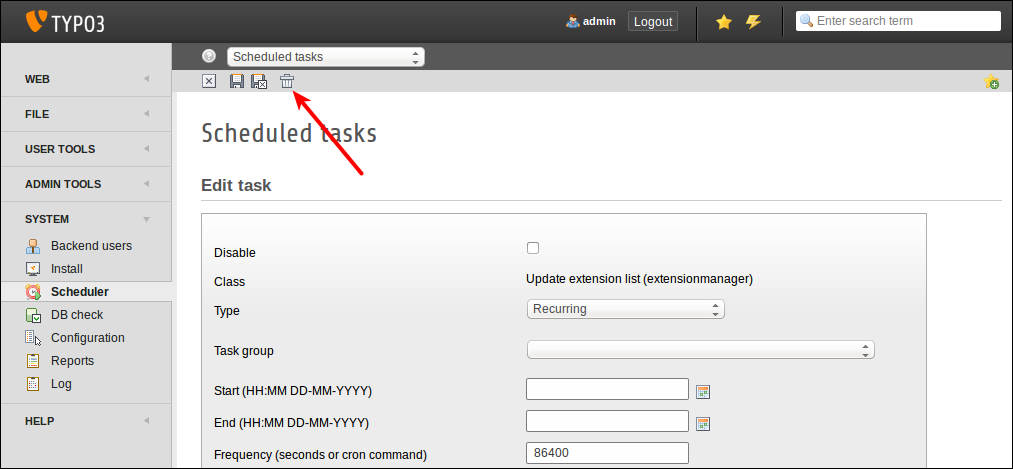
\includegraphics[width=0.95\linewidth]{Images/BackendChanges/DeleteSchedulerTaskInEditView.png}
	\end{figure}

\end{frame}

% ------------------------------------------------------------------------------
% Scheduler
% ------------------------------------------------------------------------------

\begin{frame}[fragile]
	\frametitle{Changements en Backend}
	\framesubtitle{Planificateur (2)}

	\begin{itemize}
		\item Une description peut être donnée aux tâches planifiées, elle sera affichée en sous-titre en vue liste ou en info-bulles (voir diapositive suivante)
	\end{itemize}

	\begin{figure}
		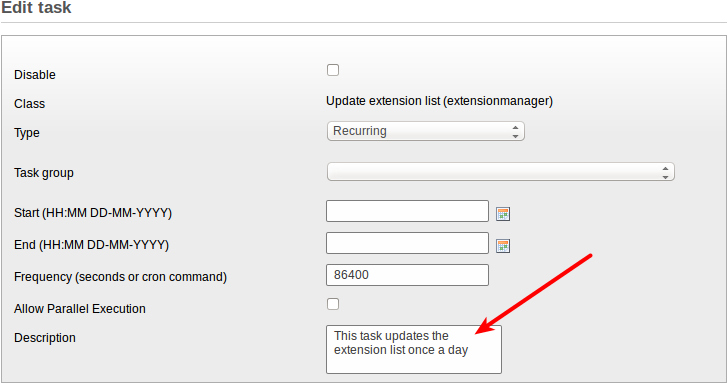
\includegraphics[width=0.7\linewidth]{Images/BackendChanges/SchedulerTaskDescription.png}
	\end{figure}

\end{frame}

% ------------------------------------------------------------------------------
% Scheduler
% ------------------------------------------------------------------------------

\begin{frame}[fragile]
	\frametitle{Changements en Backend}
	\framesubtitle{Planificateur (3)}

	\begin{itemize}
		\item Description d'une tâche en sous-titre\newline
			\small(cette fonctionnalité doit être activée dans la configuration de l'extension)\normalsize
	\end{itemize}

	\begin{figure}
		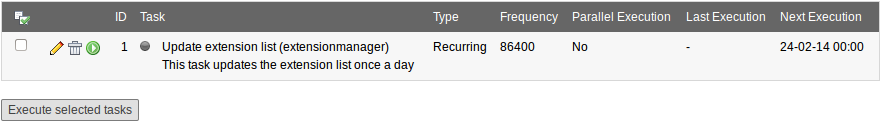
\includegraphics[width=0.95\linewidth]{Images/BackendChanges/SchedulerTaskDescriptionAsSubheader.png}
	\end{figure}

	\begin{itemize}
		\item Description de la tâche en infobulle (« hover »)
	\end{itemize}

	\begin{figure}
		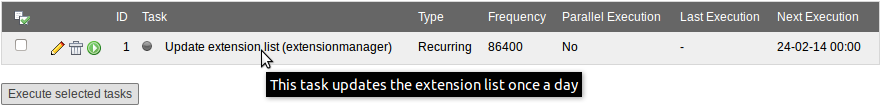
\includegraphics[width=0.95\linewidth]{Images/BackendChanges/SchedulerTaskDescriptionAsTooltip.png}
	\end{figure}

\end{frame}

% ------------------------------------------------------------------------------
% Scheduler
% ------------------------------------------------------------------------------

\begin{frame}[fragile]
	\frametitle{Changements en Backend}
	\framesubtitle{Planificateur (4)}

	\begin{itemize}
		\item Il est maintenant possible de grouper les tâches planifiées
		\item Ajout des enregistrements « Groupe de tâches planifiées » sur la page racine (UID:0) et sélection d'un groupe dans la tâche
	\end{itemize}

	\begin{figure}
		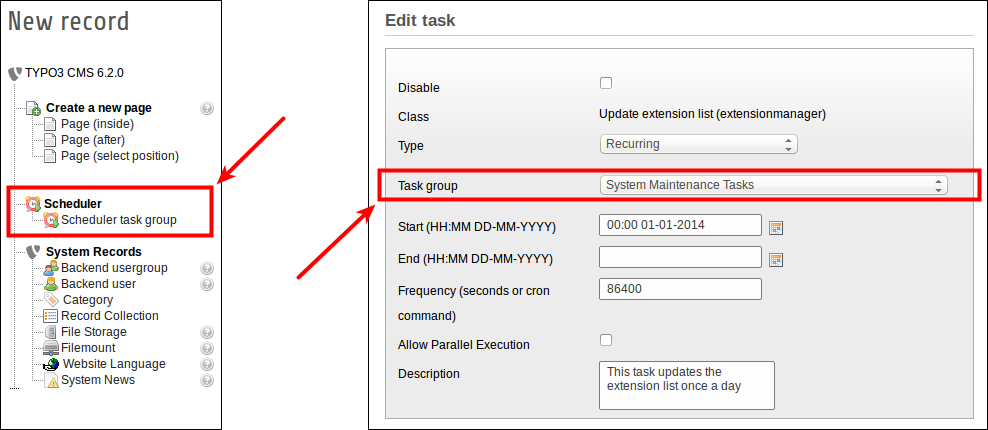
\includegraphics[width=0.85\linewidth]{Images/BackendChanges/SchedulerTaskGroup.png}
	\end{figure}

\end{frame}

% ------------------------------------------------------------------------------
% System Extension : Form
% ------------------------------------------------------------------------------
% http://forge.typo3.org/issues/38094

\begin{frame}[fragile]
	\frametitle{Changements en Backend}
	\framesubtitle{Extension système : Form}

	\begin{columns}[T]

		\begin{column}{.5\textwidth}
			\begin{itemize}
				\item Nouveau post-processor pour le cObject FORM : \textbf{redirect}\newline
					(redirection après soumission)\newline
				\item La valeur est parsée par la fonction TypoScript \texttt{typolink},\newline
					la valeur peut donc être un ID de page ou une URL
			\end{itemize}
		\end{column}

		\begin{column}{.5\textwidth}
			\begin{figure}\vspace*{-0.4cm}
				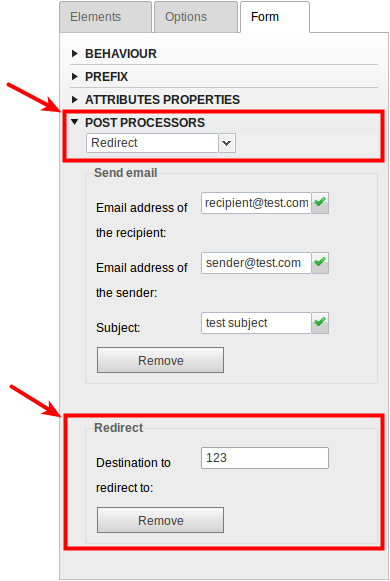
\includegraphics[width=0.65\linewidth]{Images/BackendChanges/FormRedirectPostProcessor.png}
			\end{figure}
		\end{column}

	\end{columns}
\end{frame}

% ------------------------------------------------------------------------------
% Module : List
% ------------------------------------------------------------------------------
% http://forge.typo3.org/issues/49810

\begin{frame}[fragile]
	\frametitle{Changements en Backend}
	\framesubtitle{Module Liste}

	\begin{itemize}
		\item Ajout de colonnes « UID » et « PID » en vue liste pour les non admins
	\end{itemize}

	\begin{figure}
		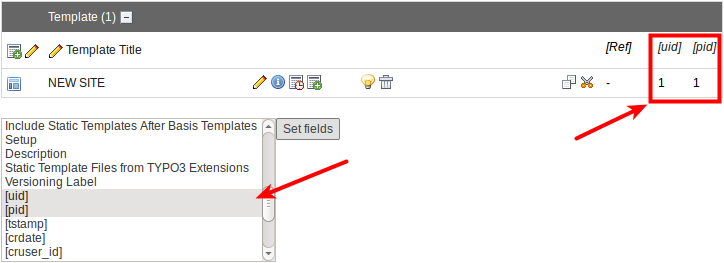
\includegraphics[width=0.95\linewidth]{Images/BackendChanges/AdditionalColumnsInListModule.png}
	\end{figure}

\end{frame}

% ------------------------------------------------------------------------------
% File Abstraction Layer
% ------------------------------------------------------------------------------
% http://forge.typo3.org/issues/50827
% http://forge.typo3.org/issues/51097

\begin{frame}[fragile]
	\frametitle{Changements en Backend}
	\framesubtitle{File Abstraction Layer}

	\begin{itemize}
		\item En cas de détection d'un fichier manquant, affichage d'un message et d'un indicateur dans l'enregistrement en base de données
		\item Le module « Rapports » l'affiche maintenant parmi les erreurs
		\item Lorsque le fichier réapparait, le message et l'indicateur sont réinitialisés
	\end{itemize}

	\begin{columns}[T]

		\begin{column}{.5\textwidth}
			\begin{figure}
				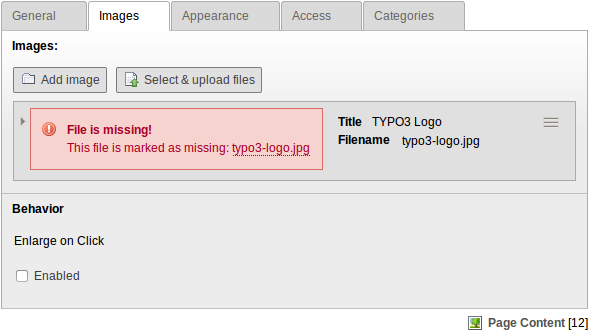
\includegraphics[width=0.95\linewidth]{Images/BackendChanges/FalMissingFileContentElement.png}
			\end{figure}
		\end{column}

		\begin{column}{.5\textwidth}
			\begin{figure}
				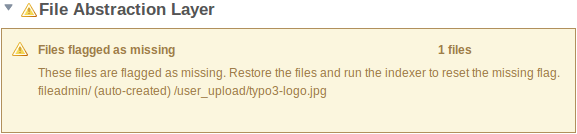
\includegraphics[width=0.95\linewidth]{Images/BackendChanges/FalMissingFileReportsModule.png}
			\end{figure}
		\end{column}

	\end{columns}

\end{frame}

% ------------------------------------------------------------------------------
% Menu/Sitemap : Categories-based Menus
% ------------------------------------------------------------------------------
% http://forge.typo3.org/issues/51161

\begin{frame}[fragile]
	\frametitle{Changements en Backend}
	\framesubtitle{Menus de catégories (1)}

	\begin{itemize}
		\item Le contenu de type « Menu/Plan du Site » peut créer un menu à partir des catégories
	\end{itemize}

	\begin{figure}
		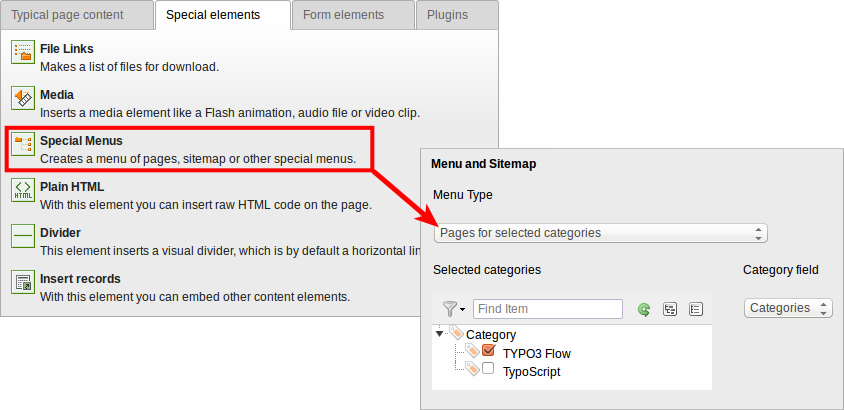
\includegraphics[width=0.8\linewidth]{Images/BackendChanges/CategoryBasedMenus.png}
	\end{figure}

\end{frame}

% ------------------------------------------------------------------------------
% Menu/Sitemap : Categories-based Menus
% (slide added in March 2014)
% ------------------------------------------------------------------------------

\begin{frame}[fragile]
	\frametitle{Changements en Backend}
	\framesubtitle{Menus de catégories (2)}

	\begin{itemize}
		\item Un autre nouveau type de menu : « \underline{Contenus} de catégories données »
	\end{itemize}

	\begin{figure}
		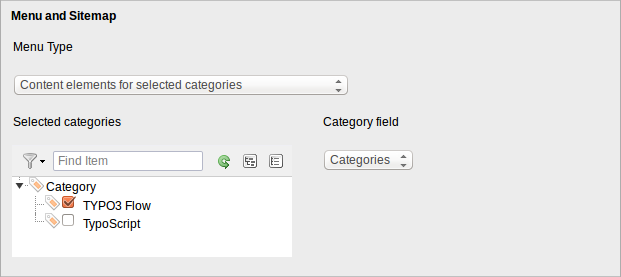
\includegraphics[width=0.6\linewidth]{Images/BackendChanges/ContentElementsForSelectedCategories.png}
	\end{figure}

\end{frame}

% ------------------------------------------------------------------------------
% Sorting Categories
% ------------------------------------------------------------------------------
% http://forge.typo3.org/issues/51590

\begin{frame}[fragile]
	\frametitle{Changements en Backend}
	\framesubtitle{Ordre des catégories}

 	\begin{itemize}
		\item Possibilité d'ordonner les catégories\newline
			(dans TYPO3 < 6.2, les catégories sont toujours classées par ordre alphabétique)
	\end{itemize}

	\begin{figure}
		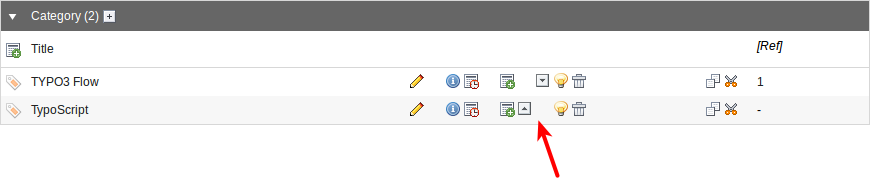
\includegraphics[width=0.95\linewidth]{Images/BackendChanges/CategorySorting.png}
	\end{figure}

\end{frame}

% ------------------------------------------------------------------------------
% Category Visibility
% ------------------------------------------------------------------------------
% http://forge.typo3.org/issues/52718

\begin{frame}[fragile]
	\frametitle{Changements en Backend}
	\framesubtitle{Visibilité des catégories}

 	\begin{itemize}
		\item La visibilité des catégories peut être restreinte à des utilisateurs BE ou à des groupes
	\end{itemize}

	\begin{figure}
		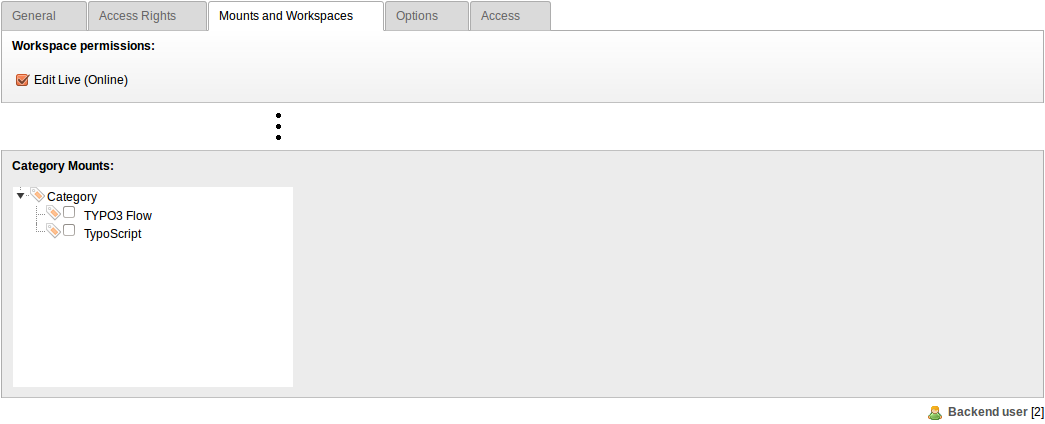
\includegraphics[width=0.95\linewidth]{Images/BackendChanges/CategoryVisibility.png}
	\end{figure}

\end{frame}

% ------------------------------------------------------------------------------
% « New Content » icon always visible
% ------------------------------------------------------------------------------
% http://forge.typo3.org/issues/48938
% http://forge.typo3.org/issues/51480

\begin{frame}[fragile]
	\frametitle{Changements en Backend}
	\framesubtitle{Utilisabilité}

 	\begin{itemize}
		\item L'icône « nouveau contenu » est toujours visible si la colonne est vide\newline
			(ce qui aide les contributeurs à comprendre ce qu'ils peuvent faire)
	\end{itemize}

	\begin{figure}
		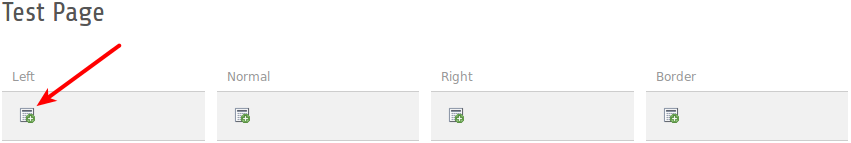
\includegraphics[width=0.95\linewidth]{Images/BackendChanges/NewContentIconAlwaysVisible.png}
	\end{figure}

\end{frame}

% ------------------------------------------------------------------------------
% Module « Functions » : Hide In Menus
% ------------------------------------------------------------------------------
% http://forge.typo3.org/issues/51017

\begin{frame}[fragile]
	\frametitle{Changements en Backend}
	\framesubtitle{Fonctions}

	\begin{itemize}
		\item A la création de plusieurs pages dans le module « fonctions », une nouvelle case à cocher permet aux contributeurs de cacher ces pages dans les menus (Très pratique lors de la création de nombreuses pages à la volée)
	\end{itemize}

	\begin{figure}
		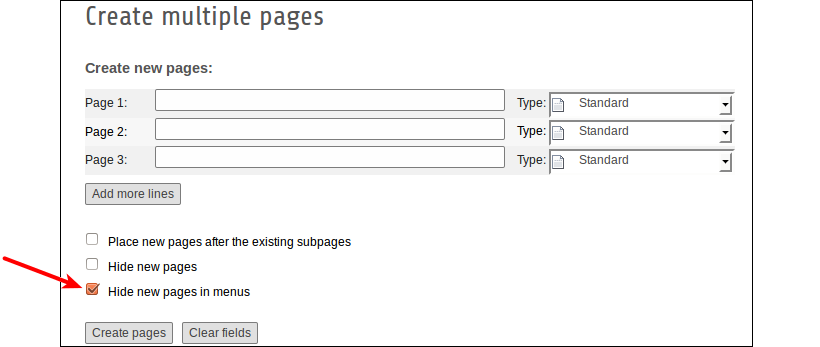
\includegraphics[width=0.85\linewidth]{Images/BackendChanges/CreateMultiplePagesHideInMenu.png}
	\end{figure}

\end{frame}

% ------------------------------------------------------------------------------
% Extension Manager : Upload Extensions
% ------------------------------------------------------------------------------
% http://forge.typo3.org/issues/51776
% http://forge.typo3.org/issues/51437

\begin{frame}[fragile]
	\frametitle{Changements en Backend}
	\framesubtitle{Gestionnaire d'extensions}

 	\begin{itemize}
		\item Télécharger une extension via la fonction « Obtenir des extensions »
	\end{itemize}

	\begin{figure}
		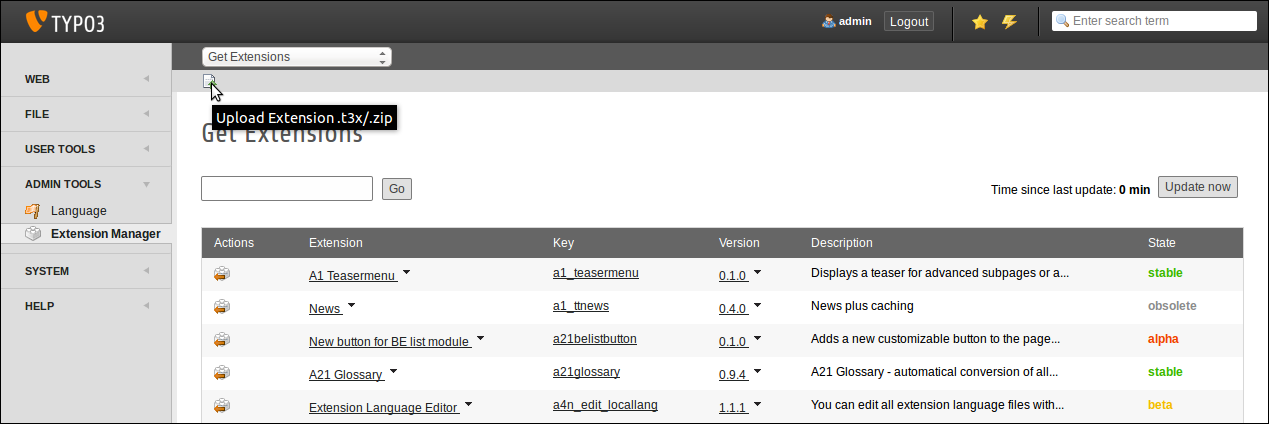
\includegraphics[width=0.95\linewidth]{Images/BackendChanges/UploadExtension.png}
	\end{figure}

\end{frame}

% ------------------------------------------------------------------------------
% Recycler
% ------------------------------------------------------------------------------
% http://forge.typo3.org/issues/52324

\begin{frame}[fragile]
	\frametitle{Backend Changes}
	\framesubtitle{Corbeille}

 	\begin{itemize}
		\item Les enregistrements de la corbeille peuvent être classés par date de dernière modification (ce qui permet aux utilisateurs de récupérer un enregistrement spécifique)
	\end{itemize}

	\begin{figure}
		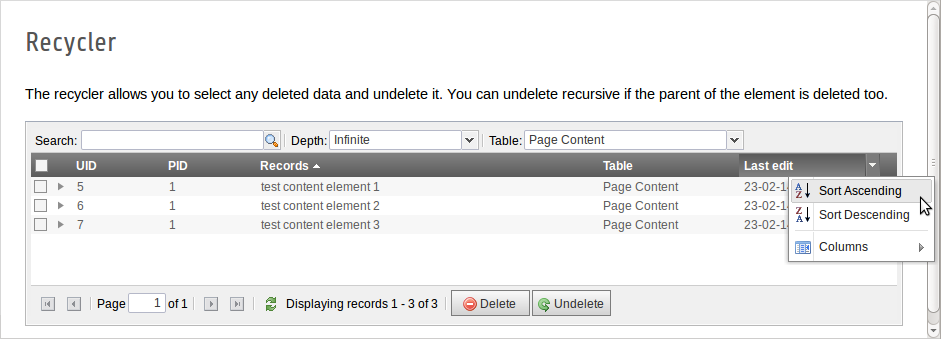
\includegraphics[width=0.95\linewidth]{Images/BackendChanges/RecyclerSortRecord.png}
	\end{figure}

\end{frame}

% ------------------------------------------------------------------------------
% File/Directory Permissions
% ------------------------------------------------------------------------------

\begin{frame}[fragile]
	\frametitle{Changements en Backend}
	\framesubtitle{Permissions Fichiers/Répertoires}

 	\begin{itemize}
		\item Plus de granularité dans la configuration des droits sur les fichiers/répertoires pour les utilisateurs BE et les groupes
			\begingroup\color{typo3red}\textbf{(1)}\endgroup
		\item Déjà possible depuis TYPO3 6.0, mais avec UserTSconfig
			\begingroup\color{typo3red}\textbf{(2)}\endgroup
	\end{itemize}

	\begin{figure}
		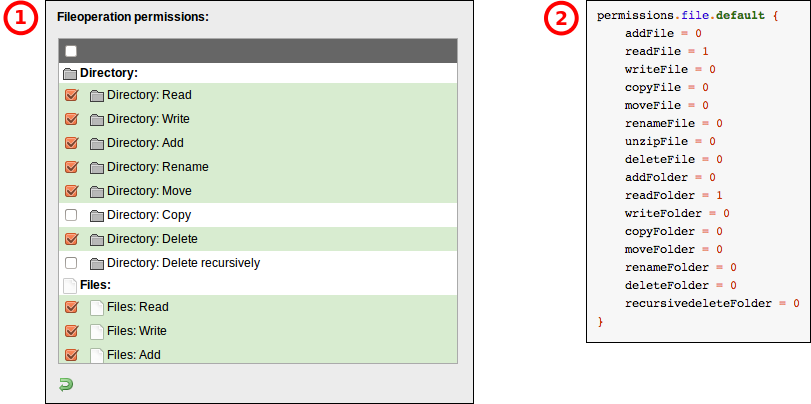
\includegraphics[width=0.75\linewidth]{Images/BackendChanges/FileAndDirectoryPermissions.png}
	\end{figure}

\end{frame}

% ------------------------------------------------------------------------------
% OpenID
% ------------------------------------------------------------------------------

\begin{frame}[fragile]
	\frametitle{Backend Changes}
	\framesubtitle{OpenID (1)}

 	\begin{itemize}
		\item L'OpenID pour l'authentification d'un utilisateur BE peut être configurée avec un assistant
		\item L'extension système « openid » est nécessaire pour activer l'assistant
	\end{itemize}

	\begin{figure}
		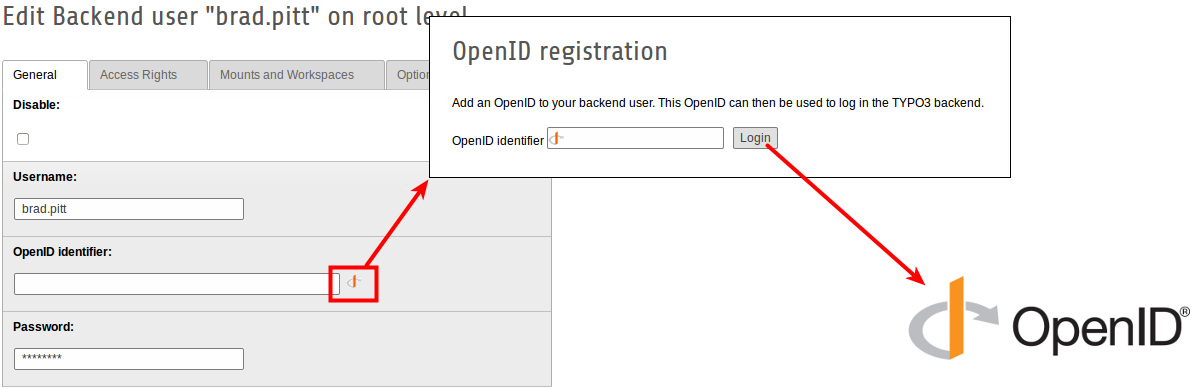
\includegraphics[width=0.95\linewidth]{Images/BackendChanges/OpenIdWizard.png}
	\end{figure}

\end{frame}

% ------------------------------------------------------------------------------
% OpenID
% ------------------------------------------------------------------------------

\begin{frame}[fragile]
	\frametitle{Changement en Backend}
	\framesubtitle{OpenID (2)}

 	\begin{itemize}
		\item La gestion de l'OpenID peut être configurée au travers d'un assistant
		\item Extension : openid (extension système) est nécessaire pour activer cet assistant
	\end{itemize}

	\begin{figure}
		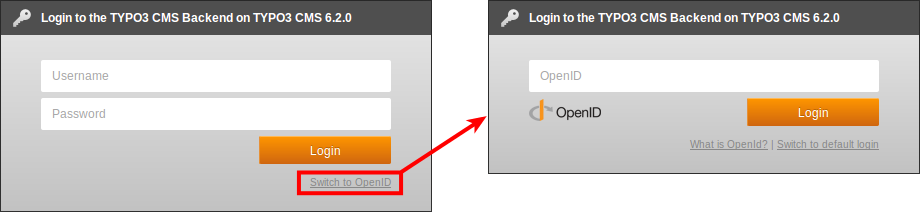
\includegraphics[width=0.8\linewidth]{Images/BackendChanges/OpenIdLogin.png}
	\end{figure}

 	\begin{itemize}
		\item En savoir plus sur l'OpenID :\newline
			\small\url{http://openid.net}\normalsize
	\end{itemize}

\end{frame}

% ------------------------------------------------------------------------------
% Workspaces
% ------------------------------------------------------------------------------
% http://forge.typo3.org/issues/50223
% http://forge.typo3.org/issues/50224

\begin{frame}[fragile]
	\frametitle{Changements en Backend}
	\framesubtitle{Workspaces}

 	\begin{itemize}
		\item Les contributeurs/utilisateurs peuvent décider à qui adresser les notifications, sans limitation système
		\item L'onglet « Tous » est maintenant visible pour \underline{tous} les utilisateurs
	\end{itemize}

	\begin{figure}
		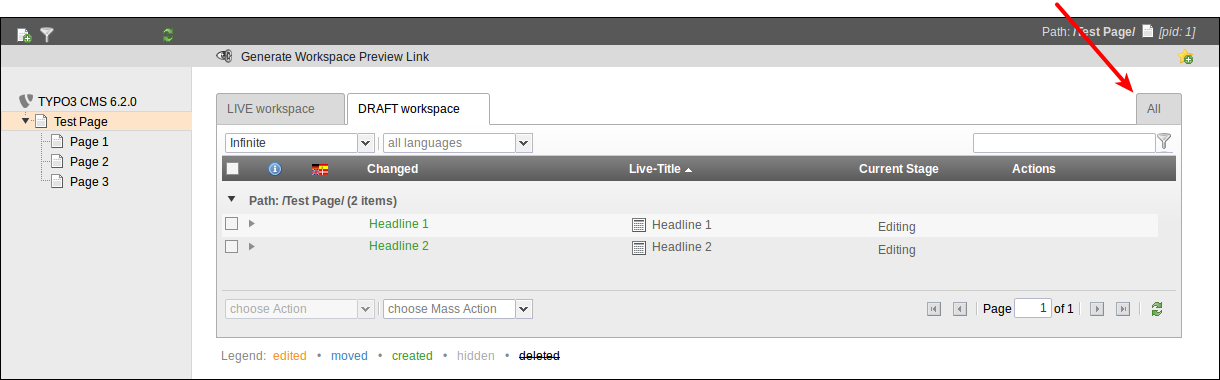
\includegraphics[width=0.95\linewidth]{Images/BackendChanges/WorkspacesTabAll.png}
	\end{figure}

\end{frame}

% ------------------------------------------------------------------------------

